\documentclass[../Livrable1.tex]{subfiles}

\begin{document}


Pour la communication sécurisée au sein du groupe, nous avons décidé d'utiliser une messagerie chiffrée, qui permet une messagerie instantanée, le partage de fichiers et la sécurisation des échanges.
Plusieurs choix se sont offerts à nous :
\begin{itemize}
    \item Notre premier était Mattermost. Nous donne l'avantage d'être open-source, compatible LDA/SSO. Son inconvénient est qu'il a une configuration complexe.
    \item Le deuxième était Rocket Chat, il est plus simple à configurer mais il est moins sécurisé que ses autres concurrents.
    \item notre 3ème option, Matrix.org à l'aide de Element, c'est le plus sécurisé et intuitif, il n'a pas d'inconvénients notables
\end{itemize}
Nous avons donc décidé de prendre la troisième option car c'était la moins contraignante en termes de mise en place avec une bonne sécurité.
Nous utilisons le client Element pour utiliser le réseau matrix.org. En effet, c'est le client qui est disponible sur le plus de plateformes.
Nous l'utilisons donc pour l'échange de mots de passe et de documents importants.
Nous utilisons avons aussi mis en place Thunderbird pour un canal de communication alternatif.
Nous avons choisi cette boîte mail chiffrée car l'ayant vu en TP chaque membre de notre groupe la maîtrise, nous avons seulement dû nous partager nos clés privées.
Pour l'échange de documents volumineux et de code, nous utilisons un dépot Github privé.
Sur le dépot Github, nous stockons les scripts utiles au projet, chiffrés à l'aide de GPG, et possiblement compréssés avec 7zip ; commme par exemple pour les images ISO.

\subsection{Exemples imagés}
\begin{figure}[h]
    \centering
    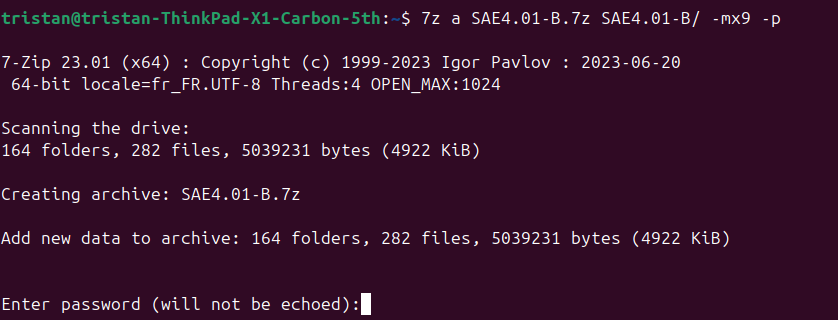
\includegraphics[width=1\textwidth]{../images/7z_chiffrer.png}
    \caption{exemple de chiffrement avec 7zip}
    \label{fig:solution1}
\end{figure}
\begin{figure}[h]
    \centering
    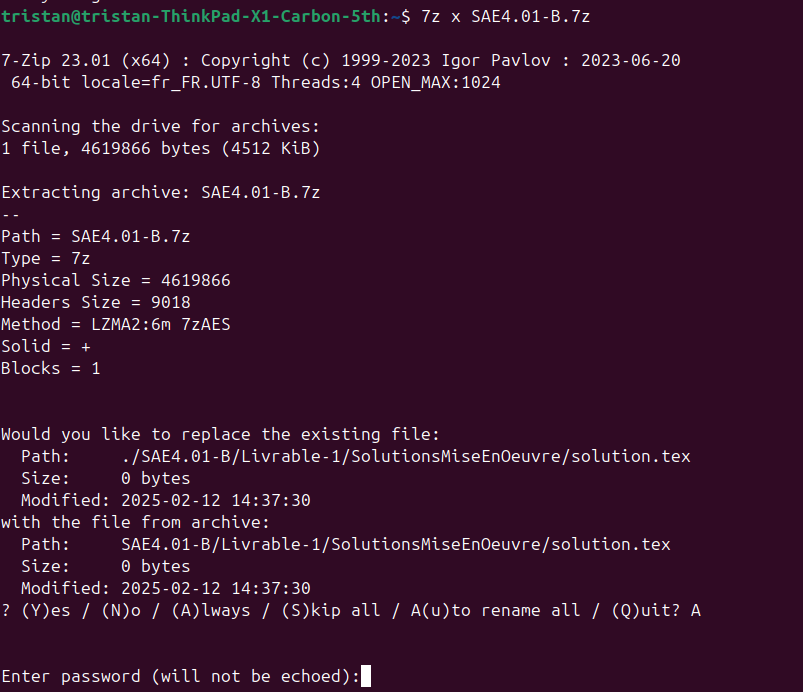
\includegraphics[width=1\textwidth]{../images/7z_dechiffr.png}
    \caption{exemple de déchiffrement avec 7zip}
    \label{fig:solution2}
\end{figure}
\begin{figure}[h]
    \centering
    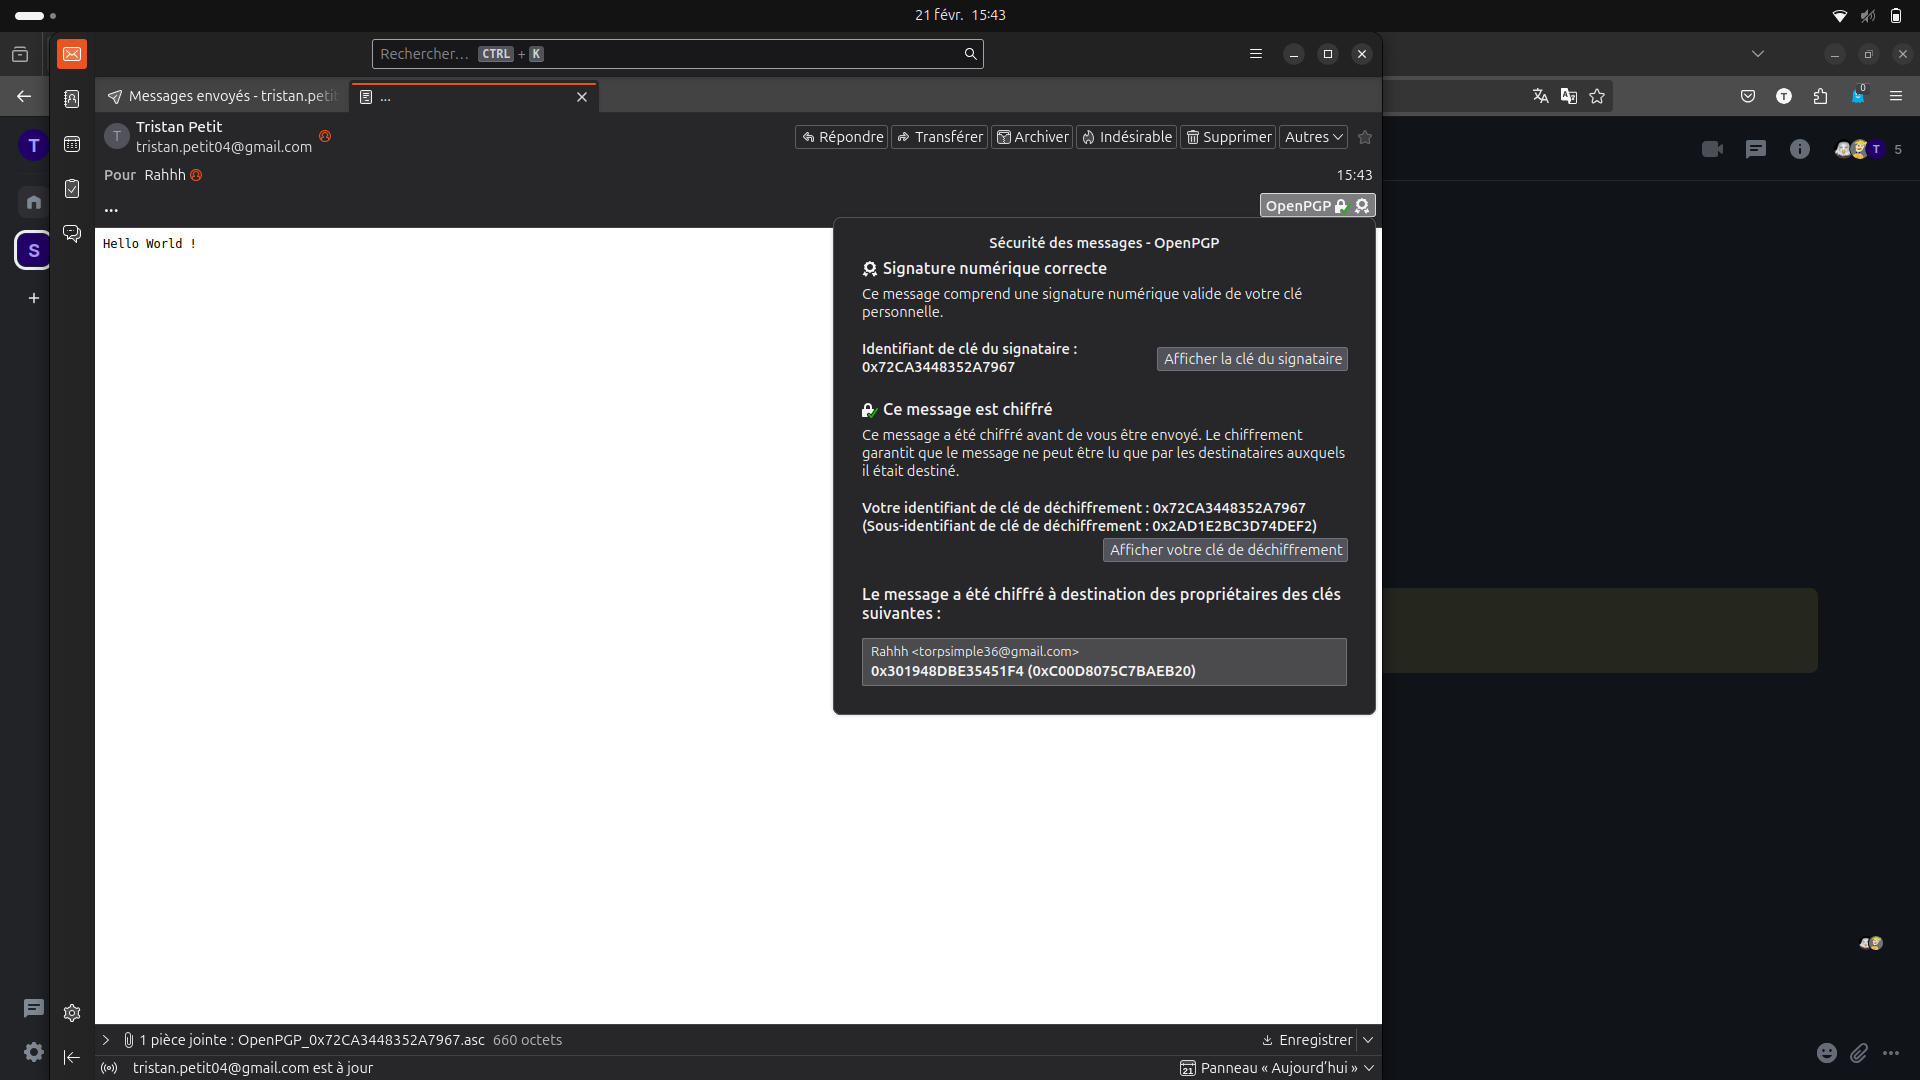
\includegraphics[width=1\textwidth]{../images/Envoi_chiffre.png}
    \caption{exemple d'envoi chiffré avec Thunderbird}
    \label{fig:solution3}
\end{figure}
\begin{figure}[h]
    \centering
    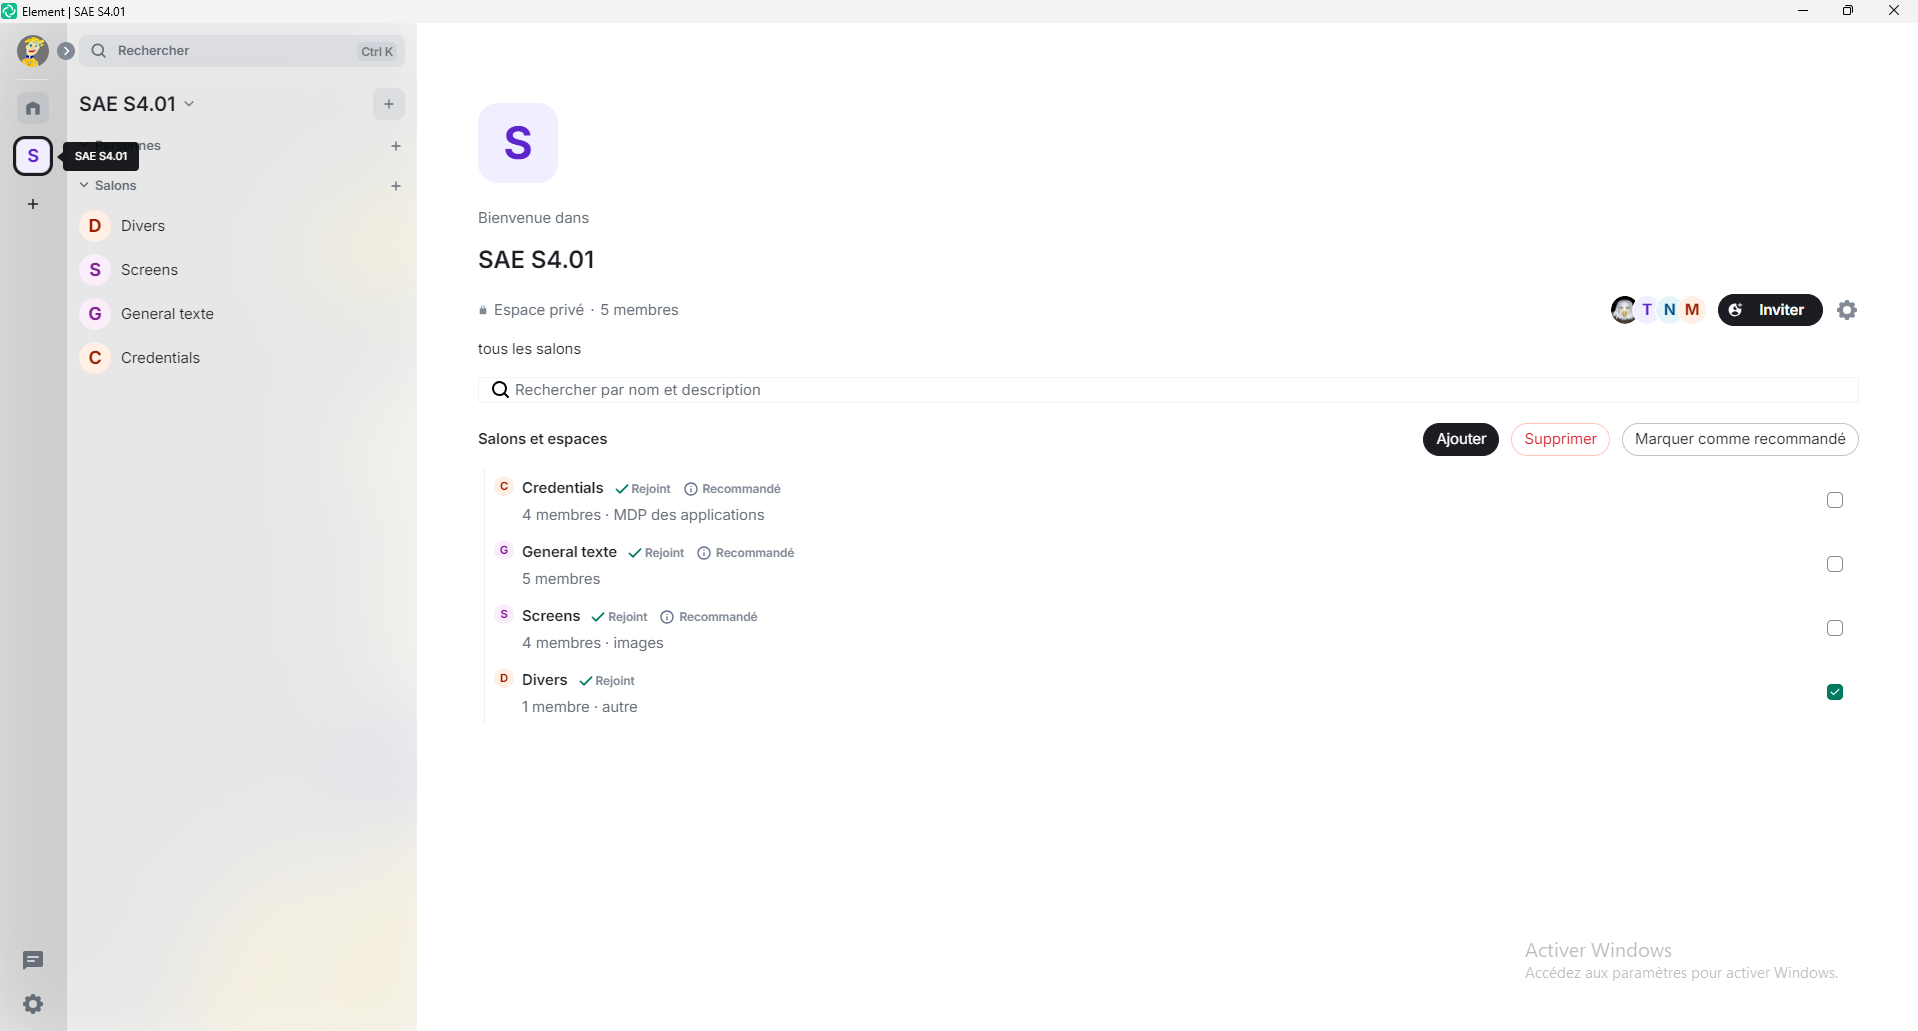
\includegraphics[width=1\textwidth]{../images/element.png}
    \caption{Espace de discussion et ses salons dans Element (matrix.org)}
    \label{fig:solution4}
\end{figure}
\end{document}
